This section will present the findings of our experiments.
The two measures we used to compare our methods are the change in loss and the change in accuracy.
The change is based on the benchmark, which is the model without any mutations.
For the further trained models, we compared the comparison model with the respective epoch of the algorithm.
For example, the results of the 1st epoch of our algorithm for a model pre-trained for 1 epoch is compared the model trained for 2 epochs, for 6 epochs it would be compared to the model trained for 7 epochs.
For the models without training, we always compared to the base accuracy and loss seen in the table \ref{tab:results}.
The data, which is shown in the following figures, doesn't describe the improvements at the endpoint of the Algorithm, but the improvements at the end of each epoch, compared to the benchmark.

\subsection{Impact of Training on Mutated Models}\label{subsec:impact-of-training-on-mutated-models}
Our models \ref{fig:loss-accuracy-training} show slightly better loss and accuracy than the benchmark during training.
For the first four epochs, the loss and accuracy of the models are significantly better than the benchmark.
We see an improvement in the median for the accuracy of 1.75\% and for the loss of 3--4\%.
Afterwards, we see a decrease of the median to the baseline of 1.
After the 11th epoch, we see a drop of the median below the baseline.
This holds also true for the loss, where we see the same drop after the 11th epoch.

For some epochs we can see an improvement to 2.5\% for the accuracy to an extreme of 7.5\%.
For the loss, we see an 12\% improvement to an extreme of 40\%.
We would attribute this to the mutation of the model and the breakage of the algorithm, as we can see in the figure \ref{fig:decay_training}.
Because we see a decrease of the data points, per epoch, after the 11th epoch, we limit all figures after this to 10 epochs, for the trained runs.
\begin{figure}
    \centering
    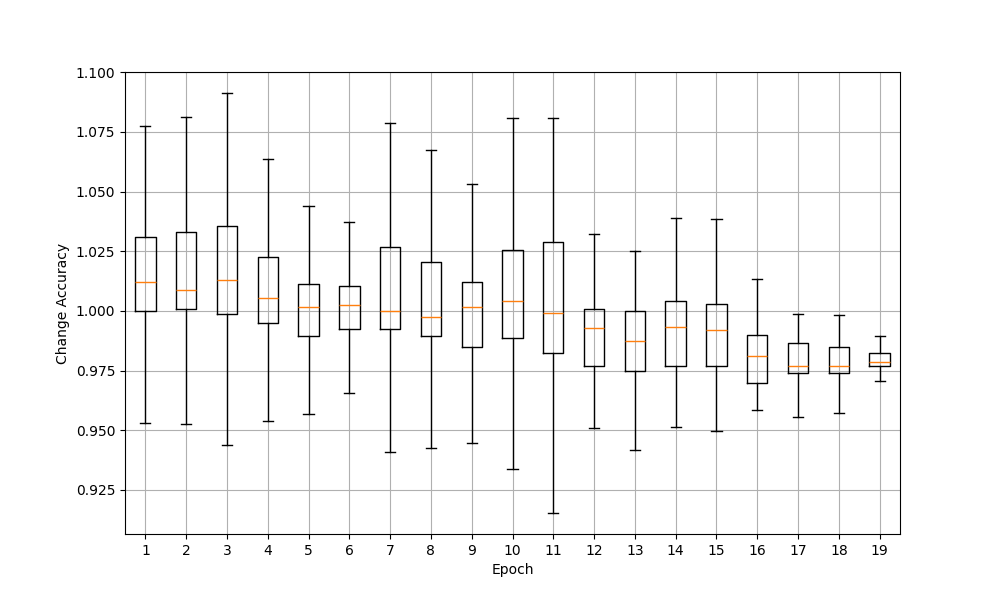
\includegraphics[width=\textwidth]{plots/Trained_Change_Acc.png}
    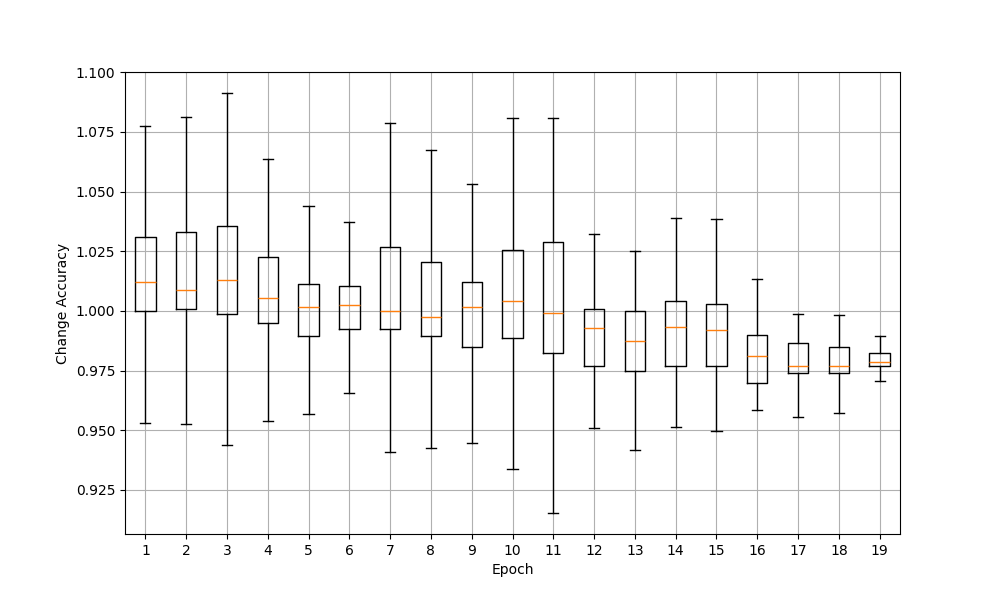
\includegraphics[width=\textwidth]{plots/Trained_Change_Loss.png}
    \caption{Loss and accuracy of the models, with training}
    \label{fig:loss-accuracy-training}
\end{figure}
\begin{figure}
    \centering
    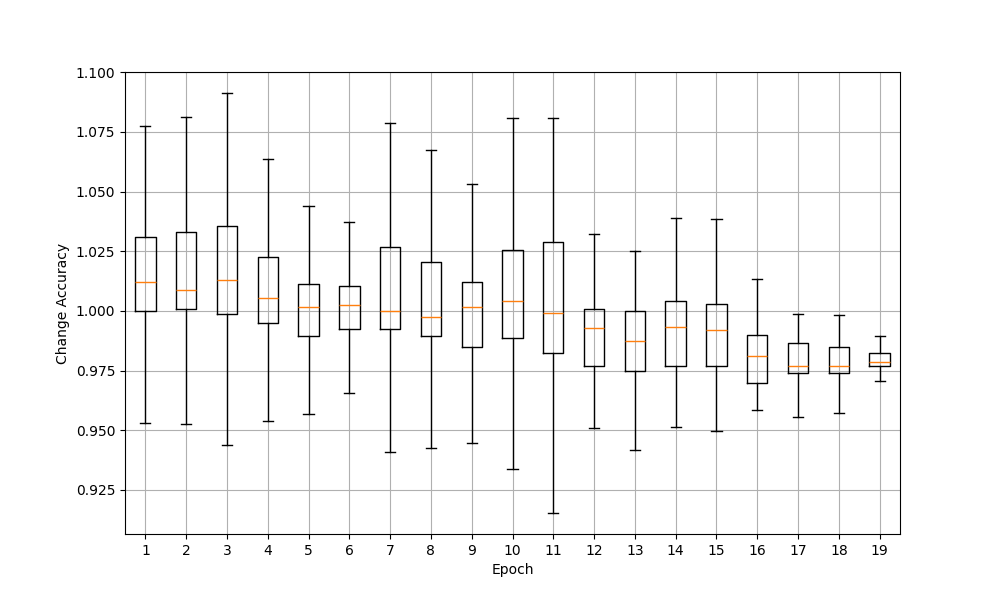
\includegraphics[width=\textwidth]{plots/Trained_Points_perEpoch.png}
    \caption{Decay of data points, per epoch, with training}
    \label{fig:decay_training}
\end{figure}
\subsection{Effects of Mutation Without Training}\label{subsec:effects-of-mutation-without-training}
As you can see in the figure \ref{fig:loss-accuracy-Notraining}, the models without training show a significant improvement in accuracy and loss during the first three epochs.
But we see only a median that isn't significantly better than the baseline of 1, for both loss and accuracy.
We see a in crease for the extremes stepwise, for each of the first 3 epochs, till we reach an improvement of 25\%, but on the other hand a decrease of -17\% on the other extreme.
The same for the loss, where we see an improvement of 45\% to a decrease of -50\%.

The three steps we are seeing, can be attributed to the comparison to only the 1st epoch, or 6th epoch respectively, so we are summing up any improvement of the model.
The reason for the sharp drop we see in the figure \ref{fig:decay_Notraining}, we would attribute to the increasing damage we are doing to the model, as we are not training it between the mutations.
Because we see a decrease of the data points, per epoch, after the 3rd epoch, we limit all figures after this to 5 epochs, for the not trained runs.
\begin{figure}
    \centering
    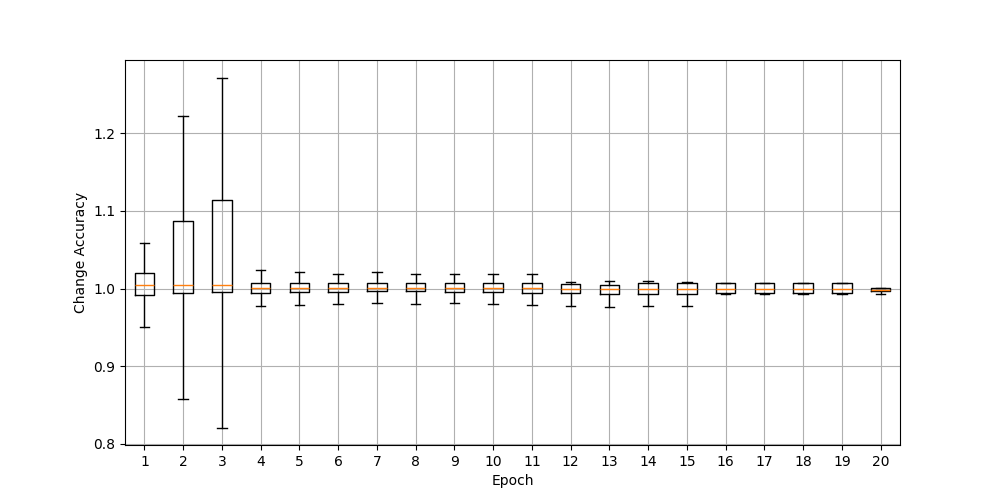
\includegraphics[width=\textwidth]{plots/NotTrained_Change_Acc.png}
    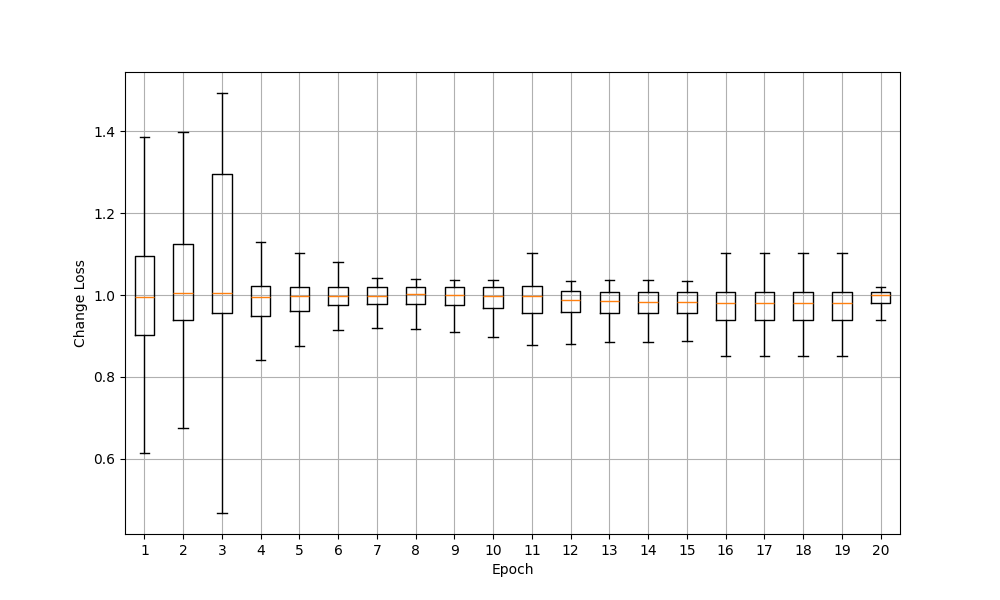
\includegraphics[width=\textwidth]{plots/NotTrained_Change_Loss.png}
    \caption{Loss and accuracy of the models, without training}
    \label{fig:loss-accuracy-Notraining}
\end{figure}
\begin{figure}
    \centering
    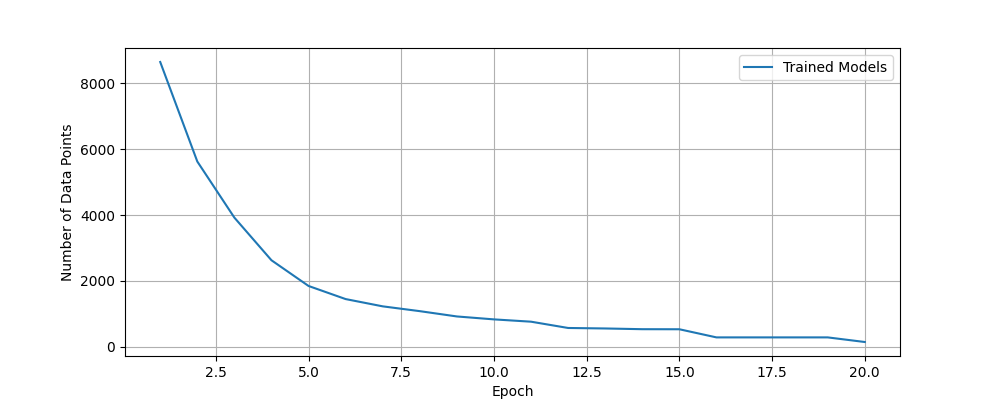
\includegraphics[width=\textwidth]{plots/NotTrained_Points_perEpoch.png}
    \caption{Decay of data points, per epoch, without training}
    \label{fig:decay_Notraining}
\end{figure}
\subsection{Effects of the extend of pre-Training}\label{subsec:effects-of-the-extend-of-pre-training}
As we can see in the figure \ref{fig:initial-epochs-notraining}, the models with 1 initial epoch show the largest potential for improvements.
While for the not trained runs, the median for loss and accuracy is not significantly better than the baseline, we can see a significant improvement for the extremes.
With a maximum improvement of 25\% for the accuracy and 45\% for the loss, for the 1st epoch.
But a decrease of up to -40\% for the accuracy and -70\% for the loss.
For the 6 initial epochs, we see a lower deviation.

For the trained runs, that can be seen in figure \ref{fig:initial-epochs-training},we see a smaller improvement over all, which is in line with the results of the previous two subsections.
But here we also see a better result for the 1 initial epoch, than for the 6 initial epochs.
But also a larger deviation for 1 initial epoch, than for the 6 initial epochs.

We would guess that the reason tHat the 1 initial epoch has more room for improvement, then the 6 initial epoch.
As we can see in the table \ref{tab:results} that the accuracy and loss of the 6 initial epochs is already better than the 1 initial epoch, at the beginning.
\begin{figure}
    \begin{subfigure}{0.5\textwidth}
        \centering
        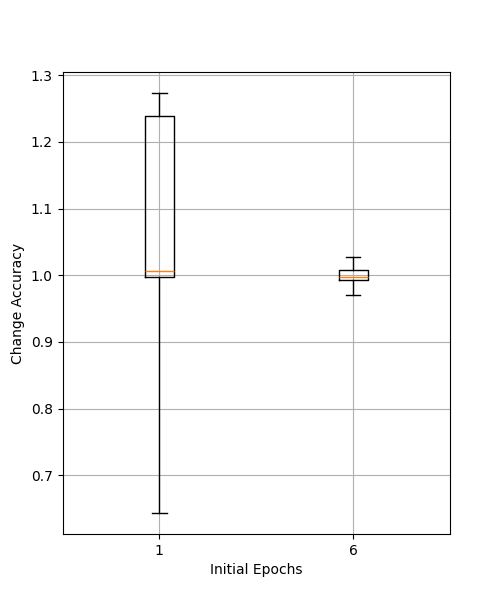
\includegraphics[width=0.95\textwidth]{plots/InitEpoch_NotTrained_accuracy.png}
    \end{subfigure}
    \begin{subfigure}{0.5\textwidth}
        \centering
        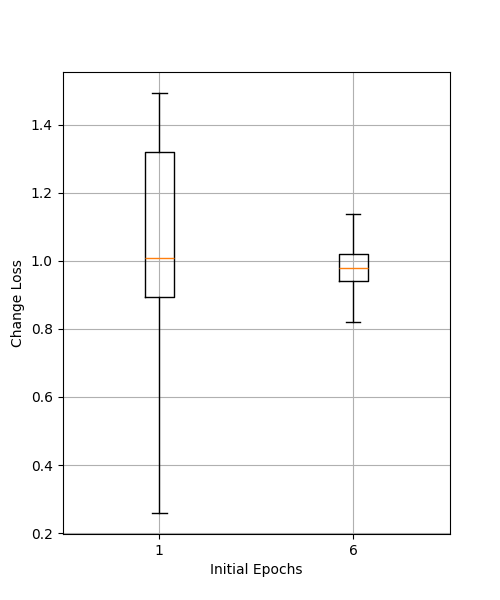
\includegraphics[width=0.95\textwidth]{plots/InitEpoch_NotTrained_loss.png}
    \end{subfigure}
    \caption{Loss and accuracy, without training, with different initial epochs}
    \label{fig:initial-epochs-notraining}
\end{figure}
\begin{figure}
    \begin{subfigure}{0.5\textwidth}
        \centering
        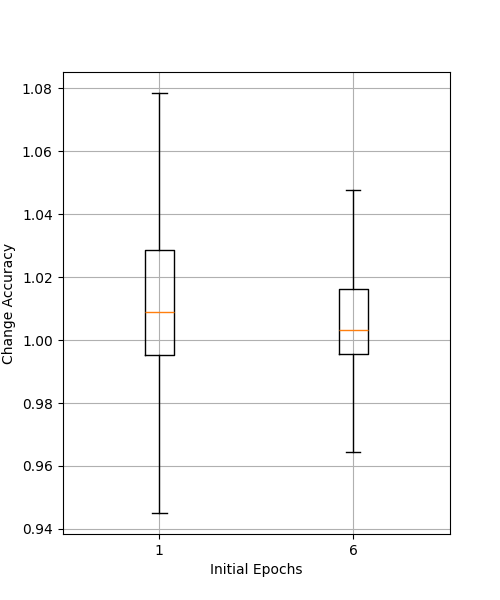
\includegraphics[width=0.95\textwidth]{plots/InitEpoch_Trained_accuracy.png}
    \end{subfigure}
    \begin{subfigure}{0.5\textwidth}
        \centering
        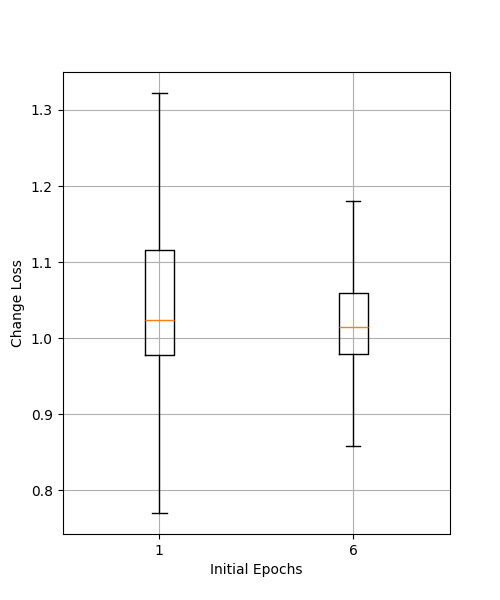
\includegraphics[width=0.95\textwidth]{plots/InitEpoch_Trained_loss.png}
    \end{subfigure}
    \caption{Loss and accuracy, with training, with different initial epochs}
    \label{fig:initial-epochs-training}
\end{figure}
\subsection{Training Dataset Size and Model Performance}\label{subsec:training-dataset-size-and-model-performance}
As you can see in the figure \ref{fig:dataset-size-notraining}, the dataset size doesn't have a significant impact on the loss and accuracy of the models without training, for the full and half dataset.
While we see a improvement for the full and half dataset, for the accuracy of often up to 25\% and for the loss a slight different result with 50\% and 30\% respectively.
For the quarter dataset we see a more negative result, while an improvement is still possible, we even see the 3rd quartile just slightly above the baseline.
And the rest all below the baseline, so roughly only a quarter of the models are better than the baseline.

For the trained runs, that can be seen in the figure \ref{fig:dataset-size-training}, we see a larger difference between the full and half dataset.
With the full dataset, we see an improvement of up to 25\% for the accuracy and 95\% for the loss.
We even see the 1st quartile above the baseline, so three quarters of the models are better than the baseline.
This holds also true for the half dataset, where we see an improvement of up to 7.5\% for the accuracy and a bit more than 25\% for the loss.
Here also the quarter dataset is the worst, with only half of the models better than the baseline.
And even that at most for 5\% for the accuracy and around 10\% for the loss.
\begin{figure}
    \begin{subfigure}{0.5\textwidth}
        \centering
        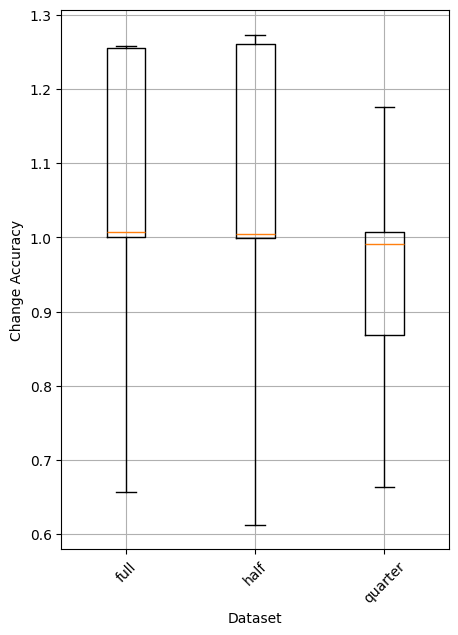
\includegraphics[width=0.95\textwidth]{plots/Dataset_NotTrained_accuracy.png}
    \end{subfigure}
    \begin{subfigure}{0.5\textwidth}
        \centering
        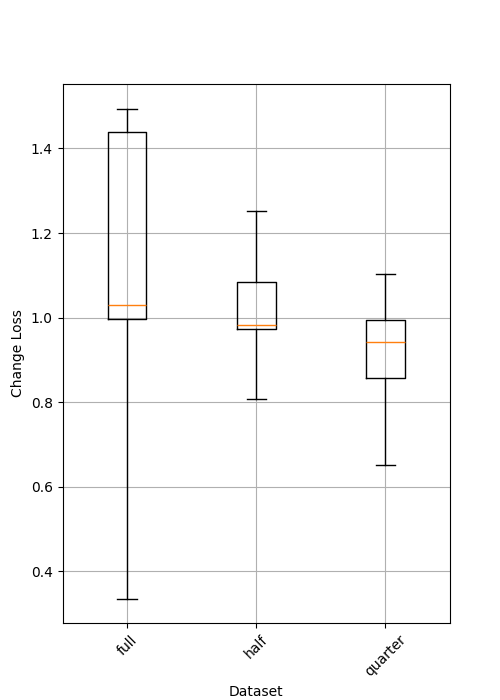
\includegraphics[width=0.95\textwidth]{plots/Dataset_NotTrained_loss.png}
    \end{subfigure}
    \caption{Loss and accuracy, without training, with different dataset sizes}
    \label{fig:dataset-size-notraining}
\end{figure}
\begin{figure}
    \begin{subfigure}{0.5\textwidth}
        \centering
        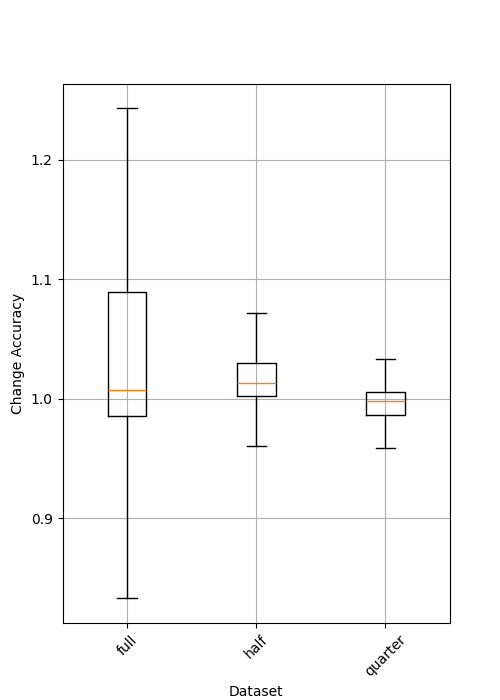
\includegraphics[width=0.95\textwidth]{plots/Dataset_Trained_accuracy.png}
    \end{subfigure}
    \begin{subfigure}{0.5\textwidth}
        \centering
        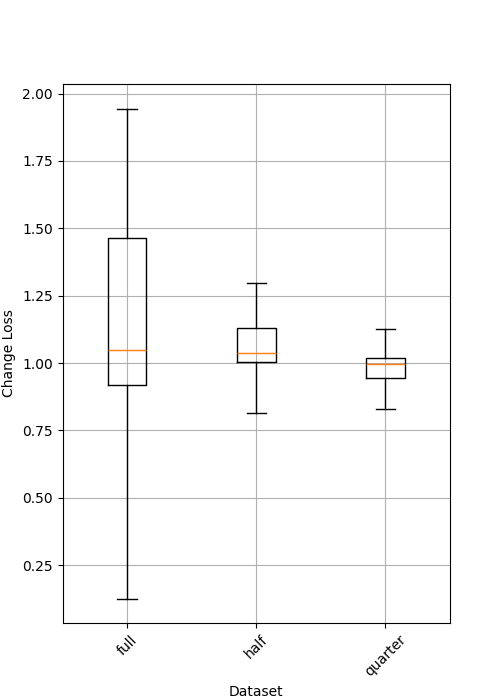
\includegraphics[width=0.95\textwidth]{plots/Dataset_Trained_loss.png}
    \end{subfigure}
    \caption{Loss and accuracy, with training, with different dataset sizes}
    \label{fig:dataset-size-training}
\end{figure}
\subsection{Influence of Suspiciousness Measures}\label{subsec:influence-of-suspiciousness-measures}
For both trained, as seen in the figure \ref{fig:suspiciousness-measures-training}, and untrained runs, as seen in the figure \ref{fig:suspiciousness-measures-notraining}, Tarantula appears to be the most promising measure of suspiciousness.
Three quarters of the models are better than the baseline, with an improvement of up to 25\% for the accuracy and 30\% for the loss, for the not trained runs and 22.5\% for the accuracy and 90\% for the loss, for the trained runs.
Ochiai seems also promising, but in contrast to Tarantula, we the third quartile is mostly below the median of tarantula, for untrained runs.
Dstar is the worst performing of the three measures, but still positive with a median slightly above the baseline, for the untrained runs.
Random performs the worst, as expected.
For the trained runs, while we see the improvements, as earlier mentioned, with Tarantula, we see no specific improvement for the other measures.
All of them having a median near the baseline, and just a slightly different deviation and both sides of the baseline.
\begin{figure}
    \begin{subfigure}{0.5\textwidth}
        \centering
        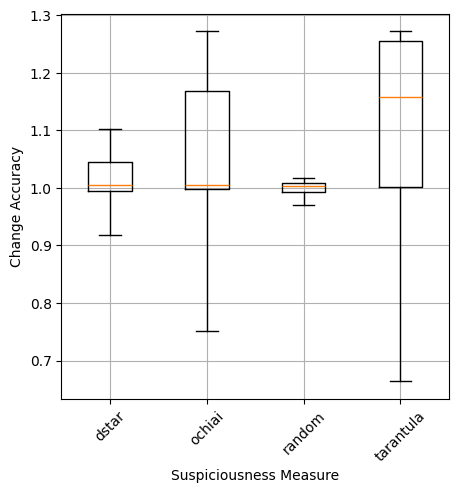
\includegraphics[width=0.95\textwidth]{plots/Meassure_NotTrained_accuracy.png}
    \end{subfigure}
    \begin{subfigure}{0.5\textwidth}
        \centering
        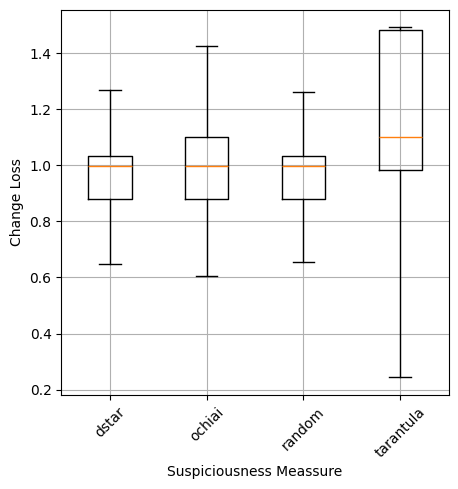
\includegraphics[width=0.95\textwidth]{plots/Meassure_NotTrained_loss.png}
    \end{subfigure}
    \caption{Loss and accuracy, without training, with different suspiciousness measures}
    \label{fig:suspiciousness-measures-notraining}
\end{figure}
\begin{figure}
    \begin{subfigure}{0.5\textwidth}
        \centering
        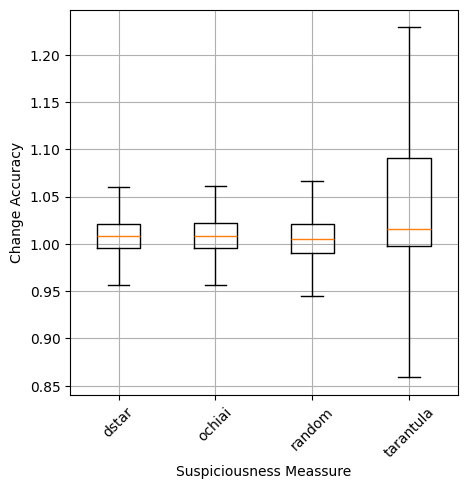
\includegraphics[width=0.95\textwidth]{plots/Meassure_Trained_accuracy.png}
    \end{subfigure}
    \begin{subfigure}{0.5\textwidth}
        \centering
        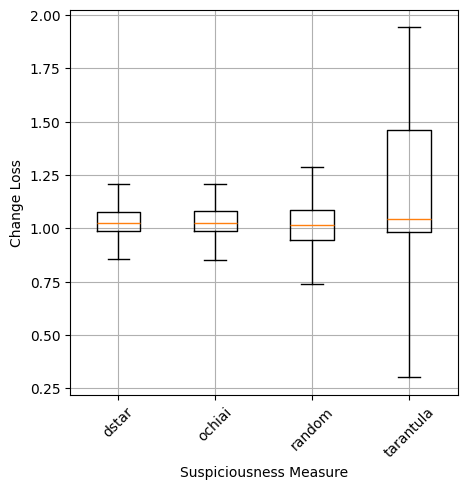
\includegraphics[width=0.95\textwidth]{plots/Meassure_Trained_loss.png}
    \end{subfigure}
    \caption{Loss and accuracy, with training, with different suspiciousness measures}
    \label{fig:suspiciousness-measures-training}
\end{figure}
\subsection{CNN vs. DNN Architectural Efficiency}\label{subsec:cnn-vs.-dnn-architectural-efficiency}
For the non-trained runs, as seen in the figure \ref{fig:architecture-notraining}, the CNN1 architecture is the most promising, with an improvement of up to 25\% for the accuracy and 35--45\% for the loss.
While CNN2 is promising for the accuracy, with an improvement of up to 10\%, it is the worst for the loss, with a worsening tendency.
The DNN models are only performing mediocre, with a median slightly above the baseline, but only slight outliers, for both loss and accuracy.
The DNN2 is slightly better than the DNN1, in both cases.

For the trained runs, as seen in the figure \ref{fig:architecture-training}, the CNN1 architecture is the most promising, with an improvement of up to 15--25\% for the accuracy and 50--90\% for the loss.
While CNN2 is mediocre for the accuracy, with an even distribution around the median at the baseline, it is the worst for the loss, with a worsening tendency.
The DNN models are only performing mediocre, with a median slightly above the baseline, but only slight outliers, for both loss and accuracy.

We aren't seeing us able to draw conclusions from the results, especially the experiments should be repeated with properly designed models and different datasets.
\begin{figure}
    \begin{subfigure}{0.5\textwidth}
        \centering
        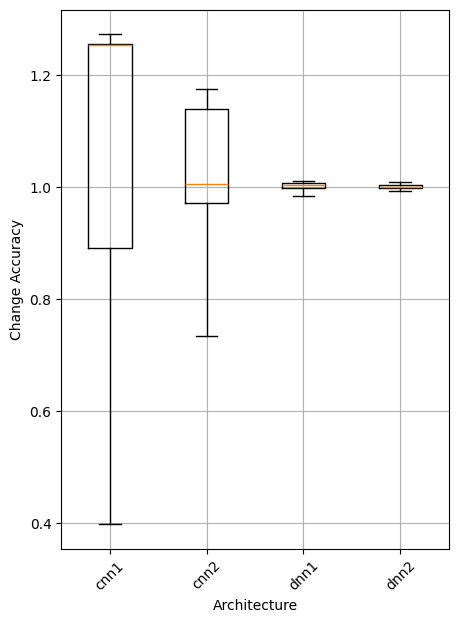
\includegraphics[width=0.95\textwidth]{plots/Architecture_NotTrained_accuracy.png}
    \end{subfigure}
    \begin{subfigure}{0.5\textwidth}
        \centering
        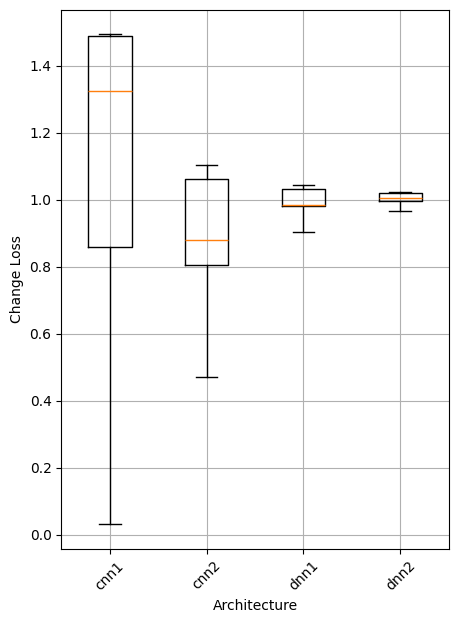
\includegraphics[width=0.95\textwidth]{plots/Architecture_NotTrained_loss.png}
    \end{subfigure}
    \caption{Loss and accuracy, without training, with different architectures}
    \label{fig:architecture-notraining}
\end{figure}
\begin{figure}
    \begin{subfigure}{0.5\textwidth}
        \centering
        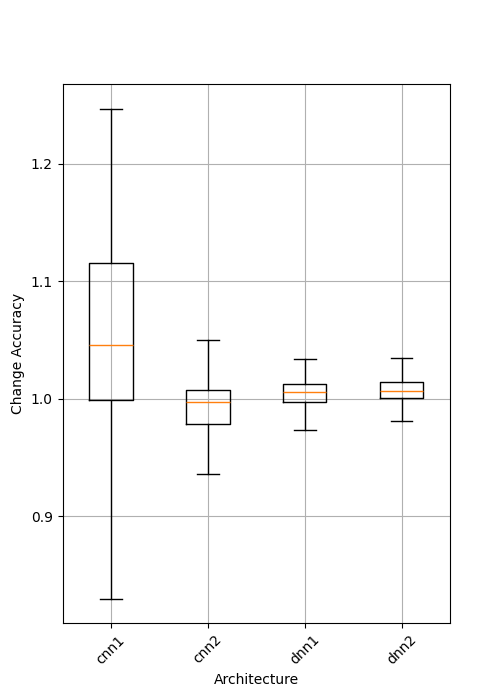
\includegraphics[width=0.95\textwidth]{plots/Architecture_Trained_accuracy.png}
    \end{subfigure}
    \begin{subfigure}{0.5\textwidth}
        \centering
        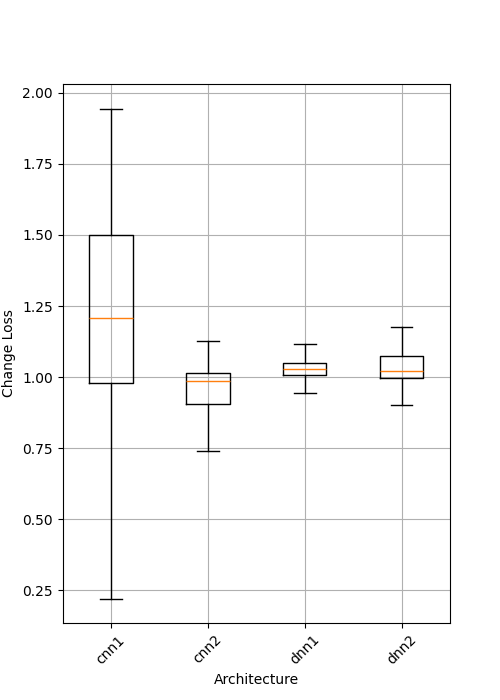
\includegraphics[width=0.95\textwidth]{plots/Architecture_Trained_loss.png}
    \end{subfigure}
    \caption{Loss and accuracy, with training, with different architectures}
    \label{fig:architecture-training}
\end{figure}
\subsection{Offset Variations in Loss and Accuracy}\label{subsec:offset-variations-in-loss-and-accuracy}
For both trained, as seen in the figure \ref{fig:offset-training}, and untrained runs, as seen in the figure \ref{fig:offset-notraining}, the offset doesn't have a significant impact on the loss and accuracy of the models.
While seeing the same median for the offset and no offset runs, we see a larger deviation for the offset runs, for both loss and accuracy.

We would attribute this to that the offset, can lead to larger improvements, because we don't stop at local extrema in training, but also we need an even worse performance, for an epoch to break the algorithm.
\begin{figure}
    \begin{subfigure}{0.5\textwidth}
        \centering
        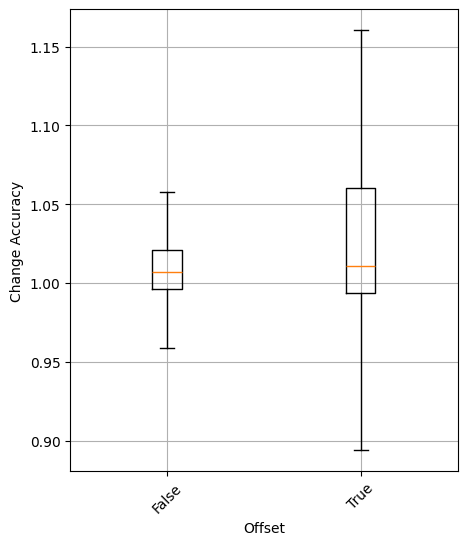
\includegraphics[width=0.95\textwidth]{plots/Offset_Trained_accuracy.png}
    \end{subfigure}
    \begin{subfigure}{0.5\textwidth}
        \centering
        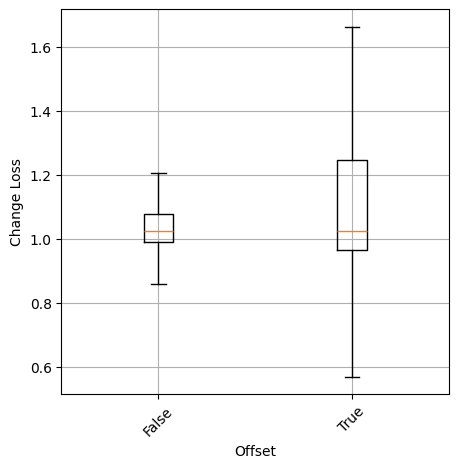
\includegraphics[width=0.95\textwidth]{plots/Offset_Trained_loss.png}
    \end{subfigure}
    \caption{Loss and accuracy, with training, with offsets or not}
    \label{fig:offset-training}
\end{figure}
\begin{figure}
    \begin{subfigure}{0.5\textwidth}
        \centering
        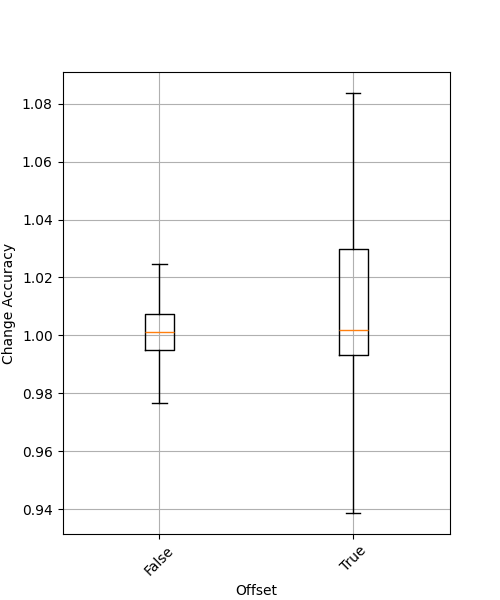
\includegraphics[width=0.95\textwidth]{plots/Offset_NotTrained_accuracy.png}
    \end{subfigure}
    \begin{subfigure}{0.5\textwidth}
        \centering
        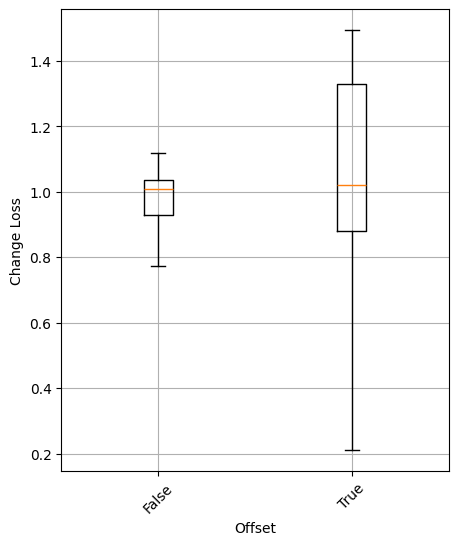
\includegraphics[width=0.95\textwidth]{plots/Offset_NotTrained_loss.png}
    \end{subfigure}
    \caption{Loss and accuracy, without training, with offsets or not}
    \label{fig:offset-notraining}
\end{figure}
\subsection{Break Conditions and Algorithm Performance}\label{subsec:break-conditions-and-algorithm-performance}
For the trained runs, as seen in the figure \ref{fig:break-conditions-training}, we see no significant differences among the four options for the different break conditions.
This holds true for both loss and accuracy.
However, for the non-trained runs, as seen in the figure \ref{fig:break-conditions-notraining}, we see some differences.
Accuracy and the Accuracy and Loss break conditions seem to be the most promising.
For both loss and accuracy, which surprised us a bit, because we would have expected the loss to be the most promising for the loss.
We see an improvement of up to 25\% for the accuracy and 30--50\% for the loss, for the Accuracy and Loss break condition, and the Accuracy break condition.
While the Loss break condition and Accuracy or Loss break condition are behaving similarly on the loss metric.
We see a slightly better performance for the Accuracy or Loss break condition, for the accuracy metric.
Which we would attribute to the fact, that the accuracy is the more important metric for the algorithm, as we are using it to decide if we are breaking the algorithm or not.
While Loss or Accuracy isn't depending on the accuracy as much as the Accuracy break condition or the Accuracy and Loss break condition.
Because also Loss alone can break the algorithm, the other two are depending on the accuracy to break the algorithm, while the last one is also depending on the loss.
\begin{figure}
    \begin{subfigure}{0.5\textwidth}
        \centering
        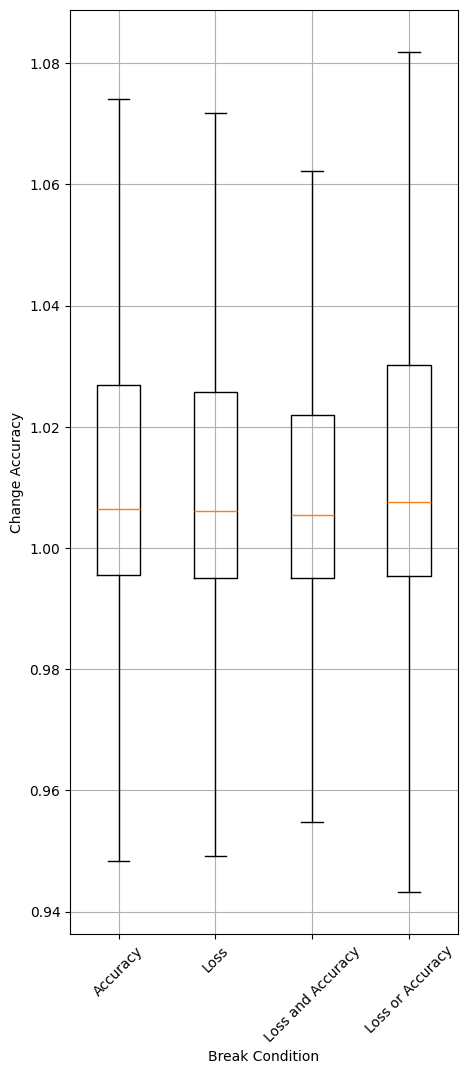
\includegraphics[width=0.95\textwidth]{plots/BreakCondition_Trained_accuracy.png}
    \end{subfigure}
    \begin{subfigure}{0.5\textwidth}
        \centering
        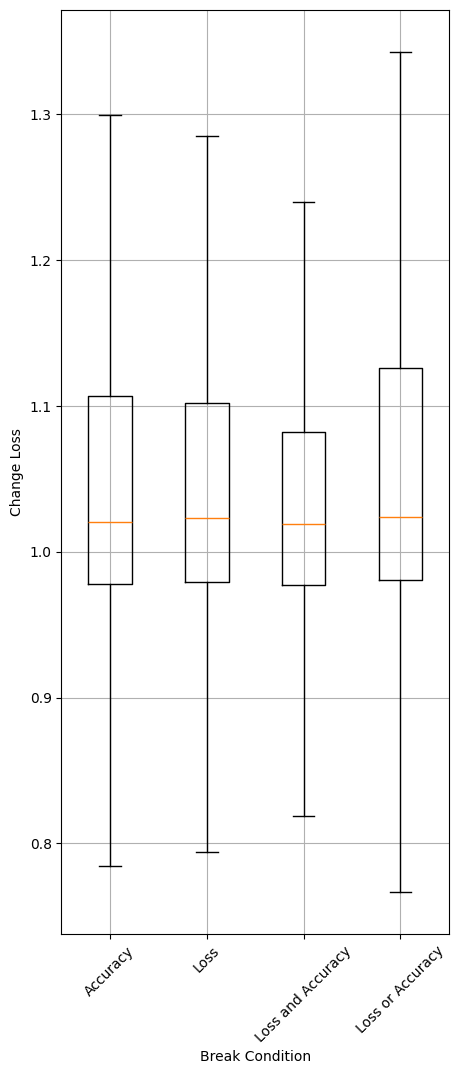
\includegraphics[width=0.95\textwidth]{plots/BreakCondition_Trained_loss.png}
    \end{subfigure}
    \caption{Loss and accuracy, with training, with different break conditions}
    \label{fig:break-conditions-training}
\end{figure}
\begin{figure}
    \begin{subfigure}{0.5\textwidth}
        \centering
        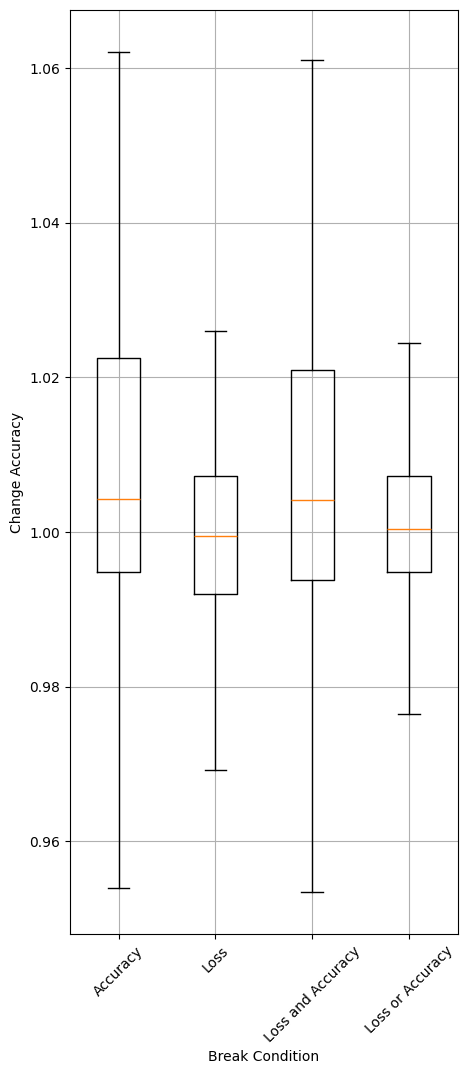
\includegraphics[width=0.95\textwidth]{plots/BreakCondition_NotTrained_accuracy.png}
    \end{subfigure}
    \begin{subfigure}{0.5\textwidth}
        \centering
        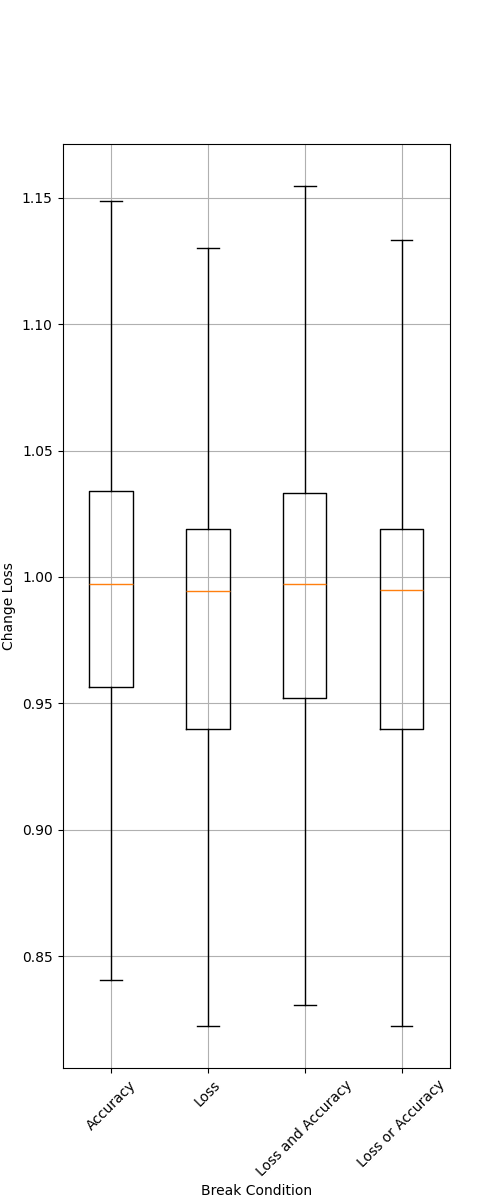
\includegraphics[width=0.95\textwidth]{plots/BreakCondition_NotTrained_loss.png}
    \end{subfigure}
    \caption{Loss and accuracy, without training, with different break conditions}
    \label{fig:break-conditions-notraining}
\end{figure}
\subsection{Contributions of Different Mutation Functions}\label{subsec:contributions-of-different-mutation-functions}
For the non-trained runs, as seen in the figure \ref{fig:mutation-functions-notraining}, we see a significant difference between the weight and bias mutation functions.
The bias functions have a median pretty close to the baseline, and a near gaussian deviation around the median.
The weight functions are looking much more promising, while we only see a median slightly above the baseline, we see for nearly all function an accuracy improvement of up to 25\%, with only the \texttt{modify\_weight\_all\_random\_by\_scalar\_gauss} function performing a bit worse.
For the loss we similar result, but we see one function standout, the \texttt{modify\_weight\_all\_random\_gauss} function, which is showing a higher improvement of around 1ß\% in comparison to the other functions.
\begin{figure}
    \begin{subfigure}{0.5\textwidth}
        \centering
        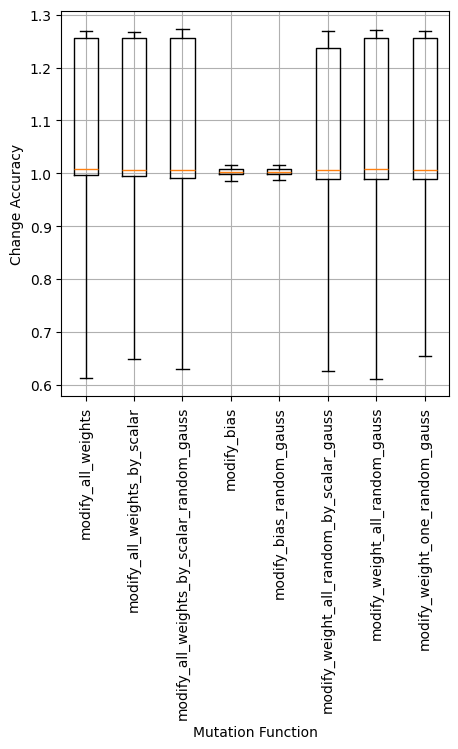
\includegraphics[width=0.95\textwidth]{plots/Mutatation_NotTrained_accuracy.png}
    \end{subfigure}
    \begin{subfigure}{0.5\textwidth}
        \centering
        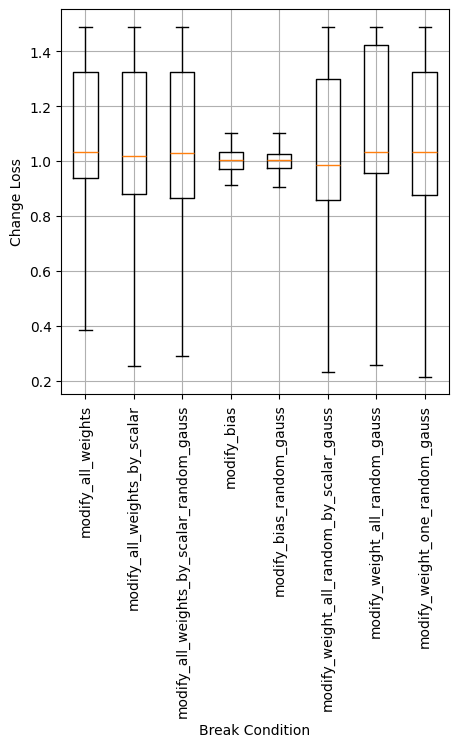
\includegraphics[width=0.95\textwidth]{plots/Mutatation_NotTrained_loss.png}
    \end{subfigure}
    \caption{Loss and accuracy, without training, with different mutation functions}
    \label{fig:mutation-functions-notraining}
\end{figure}
For the trained runs, as seen in the figure \ref{fig:mutation-functions-training}, we see a similar result, but the bias functions are performing a bit better.
All the functions are working similarly, but with the \texttt{modify\_weight\_all\_random\_by\_scalar\_gauss} function performing a bit worse.
\begin{figure}
    \begin{subfigure}{0.5\textwidth}
        \centering
        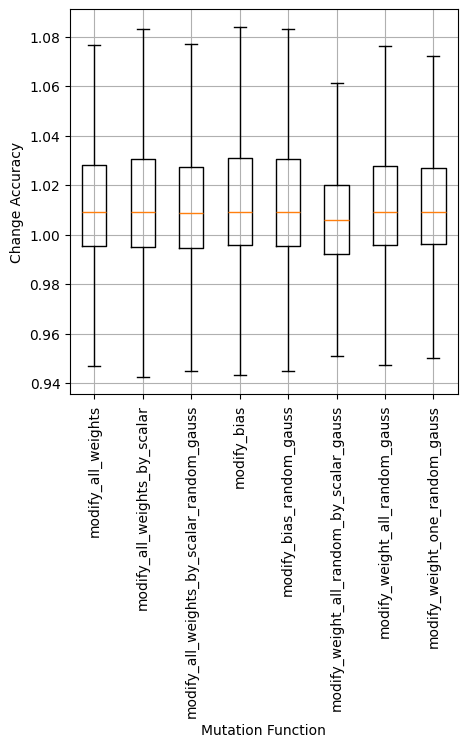
\includegraphics[width=0.95\textwidth]{plots/Mutatation_Trained_accuracy.png}
    \end{subfigure}
    \begin{subfigure}{0.5\textwidth}
        \centering
        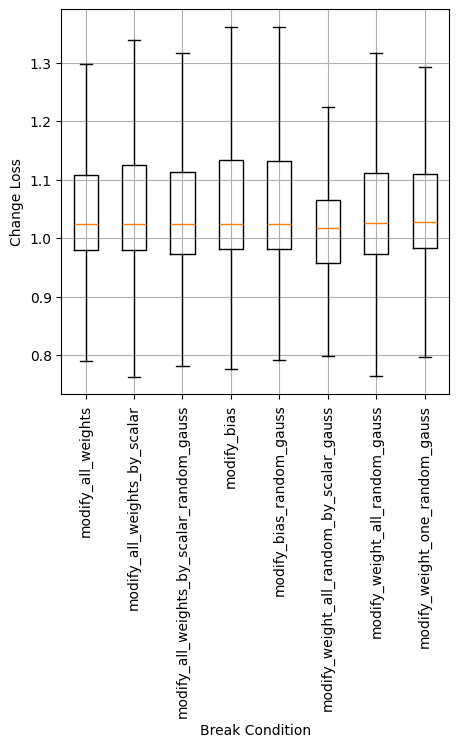
\includegraphics[width=0.95\textwidth]{plots/Mutatation_Trained_loss.png}
    \end{subfigure}
    \caption{Loss and accuracy, with training, with different mutation functions}
    \label{fig:mutation-functions-training}
\end{figure}
For both trained and untrained runs, we see no difference between the different mutation values, as seen in the figure \ref{fig:mutation-values-notraining} and \ref{fig:mutation-values-training}.
\begin{figure}
    \begin{subfigure}{0.5\textwidth}
        \centering
        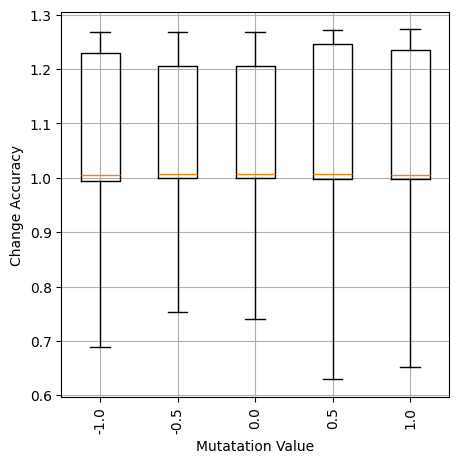
\includegraphics[width=0.95\textwidth]{plots/MutatationValue_NotTrained_accuracy.png}
    \end{subfigure}
    \begin{subfigure}{0.5\textwidth}
        \centering
        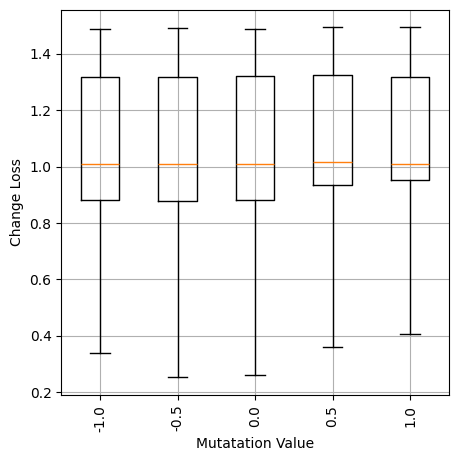
\includegraphics[width=0.95\textwidth]{plots/MutatationValue_NotTrained_loss.png}
    \end{subfigure}
    \caption{Loss and accuracy, without training, with different mutation values}
    \label{fig:mutation-values-notraining}
\end{figure}
\begin{figure}
    \begin{subfigure}{0.5\textwidth}
        \centering
        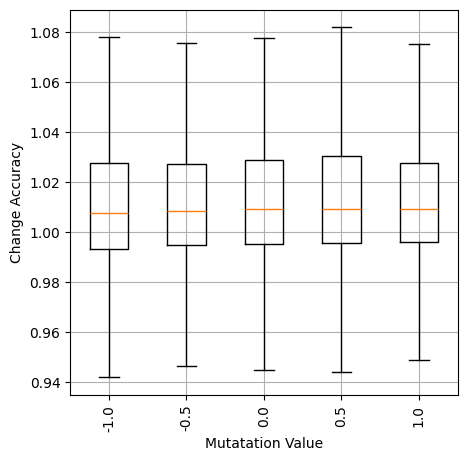
\includegraphics[width=0.95\textwidth]{plots/MutatationValue_Trained_accuracy.png}
    \end{subfigure}
    \begin{subfigure}{0.5\textwidth}
        \centering
        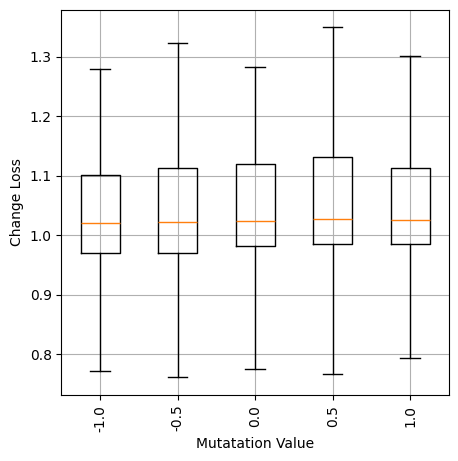
\includegraphics[width=0.95\textwidth]{plots/MutatationValue_Trained_loss.png}
    \end{subfigure}
    \caption{Loss and accuracy, with training, with different mutation values}
    \label{fig:mutation-values-training}
\end{figure}